课程设计是在给定的条件下,完成蒸汽发生器的方案设计,并进行蒸汽发生器的热力计算、水动力计算、强度计算、结构设计,然后根据所涉及的方案绘制蒸汽发生器的总图。

\subsection{给定条件}
\begin{enumerate}
    \item 蒸汽产量:$ D = 126 kg/s $
    \item 蒸汽干度:$ x = 0.99 $
    \item 蒸汽发生器的热效率:$ \eta = 0.99 $
    \item 一回路侧额定工作压力: $ p_1 = 15.0 MPa$
    \item 一回路侧设计压力:$ p_{\text{设},1} = 1.25 p_1 $
    \item 一回路侧冷却剂入口温度:$ t_{1}^{'} = 310^oC $
    \item 一回路侧冷却剂出口温度:$ t_{1}^{''} = 290^oC $
    \item 二回路侧给水温度:$ t_{f} = 220^oC $
    \item 二回路侧额定工作压力:$ p_{s} = 5 MPa $
    \item 二回路侧设计压力:$ p_{\text{设},s} = 1.25 p_{s} $
    \item 传热管壁导热系数:$ \lambda_{w} = 17.4 W/m ^oC $
    \item 传热管壁许用应力:$ [\sigma_1] = 18 kg/mm^2 $
    \item 下筒体许用应力:$ [\sigma_2] = 18 kg/mm^2 $
    \item 上筒体许用应力:$ [\sigma_3] = 18 kg/mm^2 $
    \item 球形下封头许用应力:$ [\sigma_4] = 14.5 kg/mm^2 $
    \item 管板许用应力:$ [\sigma_5] = 1800 kg/mm^2 $
    \item 传热管最小节距:$ t = 1.25 d_o $,一般取为$ 1.35 ~ 1.45 d_o $
    \item 上筒体内径$ 3200 mm $,高度$ 4000 mm $
    \item 下降空间:
          \begin{enumerate}
              \item 入口阻力系数$=1$
              \item 出口阻力系数$=1$
              \item 定位装置阻力系数$=1$
              \item 绝对粗糙度$\Delta  =0.15 mm $
          \end{enumerate}
    \item 流量分配管板:
          \begin{enumerate}
              \item 单元面积$ =533 mm^2 $
              \item 单元开孔面积$ =216 mm^2 $
          \end{enumerate}
\end{enumerate}

\subsection{蒸汽发生器的热力计算}
\begin{enumerate}
    \item 完成一回路冷却剂对传热管内壁的强迫对流放热计算,确定$ \alpha_{1} $值:
          \begin{equation*}
              \alpha = 0.023 \frac{\lambda}{d_{i}} Re_{f}^{0.8} \cdot Pr_{f}^{0.4}
          \end{equation*}
    \item 完成传热管壁的导热计算,确定管壁热阻$ R_W $ 值:
          \begin{equation*}
              R_W = \frac{d_{o}}{2\lambda_w} \ln \frac{d_{o}}{d_{i}}
          \end{equation*}
    \item 确定污垢热阻$ R_f $值:
          \begin{itemize}
              \item 对于不锈钢:$ R_f = (0.52~0.69)\times 10^{-4} \cdot m^2 \cdot ^oC / W$
              \item 对于镍基合金:$ R_f = 0.56 \times 10^{-4} \cdot m^2 \cdot ^oC / W$
          \end{itemize}
          一般污垢层厚度为$ 0.05mm $。
    \item 完成传热管外壁对二回路工质的沸腾换热计算,确定$ \alpha_2 $值:
          \begin{equation*}
              \alpha_2 = 0.557p^{0.15}q^{0.7}
          \end{equation*}
          \begin{center}
              式中:$ p \longrightarrow Pa;q \longrightarrow W/m^2 $
          \end{center}
    \item 完成传热系数$ k $值的计算:
          \begin{equation*}
              \frac{1}{k} = \frac{d_o}{d_i} \cdot \frac{1}{\aleph_i} + R_w + \frac{1}{\aleph_o} + R_f
          \end{equation*}
    \item 确定传热面积$ F $值:
          \begin{equation*}
              F = \frac{Q}{k \cdot \bigtriangleup t}
          \end{equation*}
          \begin{center}
              式中:$ Q \longrightarrow \text{传热量}; \bigtriangleup t \longrightarrow \text{传热温差} $
          \end{center}
          设计传热面积$ F_{\text{设}} = C \cdot F $
          \par 式中,$ C \longrightarrow \text{设计储备系数,一般取} C = 1.1 $
\end{enumerate}

\subsection{蒸汽发生器的水动力计算}
水动力计算主要包括:
\begin{enumerate}
    \item 一回路侧水动力计算
    \item 二回路侧循环倍率的计算
\end{enumerate}

\subsubsection{一回路侧水动力计算}
计算的具体步骤:
\begin{enumerate}
    \item 传热管内的摩擦阻力$(\bigtriangleup P_f)$
          \begin{equation*}
              \bigtriangleup P_f = \lambda \cdot \frac{H}{d_i} \cdot \frac{\rho_1u_{1}^{2}}{2}
          \end{equation*}
          \begin{align*}
              \text{式中:} & \lambda \text{—摩擦阻力系数,按有关公式或图表求取;}       \\
                            & H \text{—管子长度,}m\text{;}                             \\
                            & d_i \text{-管子直径,}m\text{;}                           \\
                            & \rho_1 \text{-一回侧路冷却剂的平均密度,} kg/m^3 \text{;} \\
                            & u_1 \text{一回侧路冷却剂的平均流速,} m/s \text{;}
          \end{align*}
          \begin{figure}[H]
              \centering
              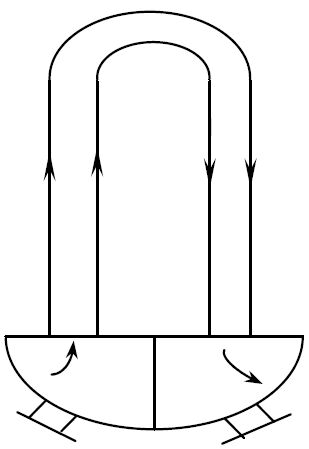
\includegraphics[width=0.3\textwidth]{一回路侧水力计算简图.jpg}
              \caption{一回路侧水力计算简图}
              \label{Fig.1}
          \end{figure}
    \item 局部阻力:$ ( \bigtriangleup P_l) $:
          \begin{equation*}
              \bigtriangleup P_l = \xi \frac{\rho_1u_{1}^{2}}{2}
          \end{equation*}
          式中:$ \xi $—局部阻力系数。$ \xi $ 值主要取决于通道的结构型式,通过实验求得,属于经验数据。
          \par 一回路侧总的局部阻力:
          \begin{equation*}
              \Delta P=\Delta P_{A}+\Delta P_{B}+\Delta P_{C}+\Delta P_{D}+\Delta P_{E}+\Delta P_{F}+\Delta P_{G}
          \end{equation*}
          其中:
          \begin{itemize}
              \item 由进口管至进口水室,通道截然突然扩大的局部阻力—$ \Delta P_A $
                    \begin{equation*}
                        \Delta P_{A}=\xi_{A} \cdot \frac{\rho_{A} \cdot u_{A}^{2}}{2}
                    \end{equation*}
              \item 在进口水室内转弯的局部阻力—$ \Delta P_B $
                    \begin{equation*}
                        \Delta P_{B}=\xi_{B} \cdot \frac{\rho_{B} \cdot u_{B}^{2}}{2}
                    \end{equation*}
              \item 由进口水室至传热管束,通道截面突然缩少的局部阻力—$ \Delta P_C $
                    \begin{equation*}
                        \Delta P_{C}=\xi_{C} \cdot \frac{\rho_{C} \cdot u_{C}^{2}}{2}
                    \end{equation*}
              \item 在$ U $型管弯头内转弯$ 180° $的局部阻力—$\Delta P_D$
                    \begin{equation*}
                        \Delta P_{D}=\xi_{D} \cdot \frac{\rho_{D} \cdot u_{D}^{2}}{2}
                    \end{equation*}
              \item 由传热管束至出口水室,通道截面突然扩大的局部阻力—$ \Delta P_E $
                    \begin{equation*}
                        \Delta P_{E}=\xi_{E} \cdot \frac{\rho_{E} \cdot u_{E}^{2}}{2}
                    \end{equation*}
              \item 在出口水室内转弯的局部阻力—$ \Delta P_F $
                    \begin{equation*}
                        \Delta P_{F}=\xi_{F} \cdot \frac{\rho_{F} \cdot u_{F}^{2}}{2}
                    \end{equation*}
              \item 由出口水室至出口接管,通道截面突然缩小的局部阻力—$ \Delta P_G $
                    \begin{equation*}
                        \Delta P_{G}=\xi_{G} \cdot \frac{\rho_{G} \cdot u_{G}^{2}}{2}
                    \end{equation*}
          \end{itemize}
          一回路侧的水阻力:$ \Delta P_H = \Delta P_f + \Delta P_l $
          \par 考虑贮备系数。其值为计算阻力的$10\%$
          \par 因此:$ \Delta P = 1.1 \Delta P_H $
\end{enumerate}

\subsubsection{二回路侧循环倍率的计算}
在设计中,常用图解法来确定循环倍率$ C_R $值和循环速度$ u_o $值。即先假定几个不同的循环倍率$ C_{R1} $、$ C_{R2} $、$ C_{R3} \cdots$值。分别计算其运动压头$ P_{m} $和总阻力$ \Delta P $,在直角坐标系里做出相应的曲线,二根曲线的交点即为稳定工况时的$ C_{R} $值,同时也可求出$ u_{o} $值。
\begin{figure}[H]
    \centering
    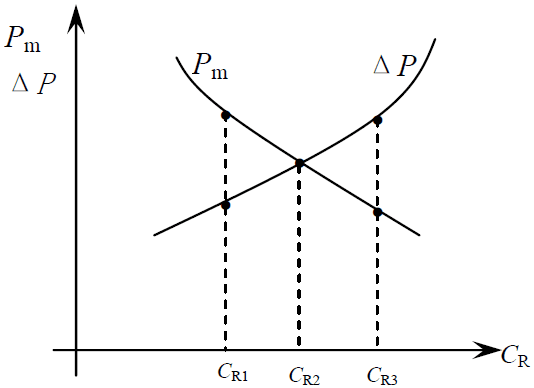
\includegraphics[width=0.5\textwidth]{用图解法计算循环倍率的曲线.png}
    \caption{用图解法计算循环倍率的曲线}
    \label{Fig.2}
\end{figure}
\begin{enumerate}
    \item 运动压头$ P_m $的计算:
          \begin{equation*}
              P_{m}=\left(\rho_{l}-\rho_{g}\right) g \varphi H_{r}
          \end{equation*}
          \begin{align*}
              \text{式中:} & H_r \text{—上升空间含汽段高度;}                         \\
                            & \rho_{l},\rho_{g} \text{—分别表示饱和水和饱和汽的密度;} \\
                            & \varphi \text{—表示上升空间平均截面含汽率。}
          \end{align*}
    \item 水循环总阻力$ \Delta P $的计算:
          \begin{align*}
               & \text{总阻力} \Delta P = \Delta P_d + \Delta P_r +\Delta P_s                                                         \\
               & \text{其中:} \Delta P_d \text{、} \Delta P_r \text{和}\Delta P_s \text{—分别表示下降空间、上升空间和分离器的阻力。} \\
               & \text{一般} \Delta P_d \approx 10\% \Delta P \text{,} \Delta P_s 由实验确定                                         \\
               & \text{而} \Delta P_{r}=\Delta P_{f}+\Delta P_{l}+\Delta P_{b}+\Delta P_{a}
          \end{align*}
          式中: $ \Delta P_{f} $ ,$ \Delta P_{l} $ ,$ \Delta P_{b} $ ,和 $ \Delta P_{a} $分别表示摩擦阻力、局部阻力、弯头区阻力和加速度阻力,可按相应的公式进行计算。
\end{enumerate}


\subsection{蒸汽发生器的强度计算}
主要内容有:
\begin{enumerate}
    \item 传热管的强度计算
    \item 筒体的强度计算
    \item 封头的强度计算
    \item 管板的强度计算
\end{enumerate}

\subsubsection{传热管的强度计算}
计算管壁厚度:
\begin{equation*}
    S^{\prime}=\frac{P_{\text {设 }} \cdot d_{0}}{200[\sigma]+0.8 P_{\text {设 }}} \cdot \varphi \cdot \phi_{R}
\end{equation*}
\begin{align*}
    \text{式中:} & P_{\text{设}} \text{—设计压力} (kg/cm^2)               \\
                  & d_o \text{—管子外径} (mm)                              \\
                  & [\sigma] \text{—许用应力}                              \\
                  & \varphi \text{—负公差修正系数,一般取} \varphi = 1.102 \\
                  & \phi_R \text{—弯曲减薄系数}                            \\
                  & \phi_{R}=1+\frac{d_{o}}{4 R}                           \\
                  & \text{式中:R—弯曲半径,取最小节圆半径。}
\end{align*}

\subsubsection{筒体的强度计算}
计算筒体厚度
\begin{equation*}
    S^{\prime}=\frac{P_{\text {设}} \cdot D_{i}}{200[\sigma]-1 \cdot 2 P_{\text {设}}} (mm)
\end{equation*}
式中:$D_i$—筒体内径$ (mm) $

\subsubsection{封头的强度计算}
计算壁厚
\begin{equation*}
    S^{\prime}=\frac{P_{\text {设 }} \cdot D_{o}}{400[\sigma]+1 \cdot 6 P_{\text {设 }}} (mm)
\end{equation*}
式中:$ D_o $—球型封头外径$ (mm) $

\subsubsection{管板的强度计算}
计算壁厚
\begin{equation*}
    S^{\prime}=\frac{1}{2} \cdot F \cdot D \sqrt{\frac{P_{i z}}{[\sigma]}} (mm)
\end{equation*}
\begin{align*}
    \text{式中:} & F \text{—系数,查TEMA 标准}F=1.04 \\
                  & D \text{—水压部分直径} (mm)
\end{align*}

\subsection{蒸汽发生器的结构设计}
主要完成下列工作:
\begin{enumerate}
    \item 管束组件的结构设计
    \item 衬筒的结构设计
    \item 下筒体结构设计
    \item 管板
    \item 分离器组件
    \item 给水管装置
    \item 排污装置
\end{enumerate}

\subsubsection{管束组件的结构设计}
确定流程数,完成传热管的排列,确定管束直径及高度,最佳高-径比一般取为3;确定管子的固定支撑,确定隔板的数目和结构。

\subsubsection{衬筒的结构设计}
确定衬筒的几何形状和尺寸。
\par 衬筒内径:$ D_{w i}=D_{\text {管束 }}+2 \delta_{t} $
\par 式中:$ \delta_t $为装配间隙,约$ 10 \sim 20 mm $。
\par 衬筒外径:$ D_{w o}=D_{w i}+2 \delta $
\par 式中:$ \delta $为衬筒壁厚,约$ 12 mm $。

\subsubsection{下筒体结构设计}
下筒体内径 $ D_{i, \text{下}}=D_{w o}+2 B $
\par 式中:$ B $为下降流道宽度,取为$ 88 mm $。

\subsubsection{管板}
确定开孔数及有关几何尺寸,确定堆焊层与筒体的连接。

\subsubsection{分离器组件}
采用三级汽水分离方式,但不做详细设计,其相应于循环倍率为$ 3,4,5 $时的流动阻力人为设定为$ 12600Pa,14900Pa,17090Pa $。
\subsubsection{给水管装置}
确定给水管的结构,布置及有关几何尺寸。

\subsubsection{排污装置}
确定排污管的结构、布置及有关几何尺寸。